\documentclass{llncs}
\usepackage[utf8]{inputenc}
\usepackage{amsmath}
\usepackage{amsfonts}
\usepackage{amssymb}
\usepackage{graphicx}
\usepackage[space]{grffile}
\graphicspath{figures/}
\usepackage{import}
\usepackage{url}
\usepackage{hyperref}
% http://tex.stackexchange.com/questions/57865/how-to-use-multiple-urls-for-one-bibtex-reference
\let\URL\url
\makeatletter
\def\url#1{\@URL#1||\@nil}
\def\@URL#1|#2|#3\@nil{%
  \URL{#1}\ifx\relax#2\relax\else| \URL{#2}\fi}
\makeatother

\usepackage{subcaption}
\usepackage{tikz}
\usepackage{siunitx}
\usepackage[disable]{todonotes}%
\let\OldTodo\todo
\renewcommand{\todo}{\OldTodo}%[inline]}
\newcommand{\todolater}[1]{\todo{#1}}%{}%
\RequirePackage[date=terse, isbn=true, doi=true, url=false, urldate=iso8601, maxbibnames=9, backref=false, backend=bibtex, style=ieee]{biblatex}
\addbibresource{securityupdates.bib}
\renewcommand{\bibfont}{\small}

\AtEveryBibitem{% Clean up the bibtex rather than editing it
 \clearname{editor} % remove editors
}

\newcommand{\daNumDataPoints}{153 Billion}
\newcommand{\daNumStartedApps}{122\,000}
\newcommand{\daNumInstalledApps}{175\,000}
\newcommand{\daNumVulnsUsed}{11}
\newcommand{\daSigNumDevices}{100}
\newcommand{\daSigNumDays}{100}
\newcommand{\daNumManufacturers}{261}
\newcommand{\daNumSigManufacturers}{9}
\newcommand{\daNumModels}{2\,380}
\newcommand{\daNumSigModels}{15}
\newcommand{\daOSVersionPercValidLines}{99.5\%}
\newcommand{\daOSTotalDaysData}{1\,140\,000}
\newcommand{\daMeanInsecurityPerc}{$87.3 \pm 0.0\%$}
\newcommand{\daMeanOutstandingVulnerabilities}{0.637}
\newcommand{\daUpdatedness}{$0.0558 \pm 0.0002$}
\newcommand{\daSecurityScore}{$2.75 \pm 0.00$}
\newcommand{\daNumFullVersions}{1\,140}
\newcommand{\daNumOSVersions}{45}
\newcommand{\daNumSigOSVersions}{23}
\newcommand{\daNumAPIVersions}{15}
\newcommand{\daNumFullVersionUpdates}{4\,220}
\newcommand{\daNumOSVersionUpdates}{3\,560}
\newcommand{\daNumFullOnlyVersionUpdates}{640}
\newcommand{\daNumSecurityUpdates}{1\,110}
\newcommand{\daNumPossibleSecurityUpdates}{2\,140}
\newcommand{\daTabSecScoresmanufacturer}{\begin{table} \centering \begin{tabular}{l|c|c|c|c} Name & $f$ & $u$ & $m$ & \textbf{Security score} \\ &&&& (out of 10) \\ \hline LG & $0.12 \pm 0.00$ & $0.32 \pm 0.00$ & 0.74 & $3.38 \pm 0.01$ \\  Motorola & $0.16 \pm 0.00$ & $0.13 \pm 0.00$ & 0.77 & $2.93 \pm 0.01$ \\  other & $0.13 \pm 0.00$ & $0.06 \pm 0.00$ & 0.64 & $2.75 \pm 0.00$ \\  Samsung & $0.14 \pm 0.00$ & $0.05 \pm 0.00$ & 0.71 & $2.67 \pm 0.00$ \\  Sony & $0.13 \pm 0.00$ & $0.18 \pm 0.00$ & 1.02 & $2.64 \pm 0.01$ \\  HTC & $0.14 \pm 0.00$ & $0.09 \pm 0.00$ & 0.89 & $2.55 \pm 0.00$ \\  asus & $0.15 \pm 0.00$ & $0.56 \pm 0.01$ & 6.06 & $2.30 \pm 0.02$ \\  Symphony & $0.00 \pm 0.00$ & $0.04 \pm 0.00$ & 4.79 & $0.19 \pm 0.00$ \\  walton & $0.00 \pm 0.00$ & $0.04 \pm 0.00$ & 5.79 & $0.14 \pm 0.01$ \\ \end{tabular} \caption{Security scores for manufacturers} \label{tab:sec_manufacturer} \end{table}}
\newcommand{\daTabSecScoresmodel}{\begin{table} \centering \begin{tabular}{l|c|c|c|c} Name & $f$ & $u$ & $m$ & \textbf{Security score} \\ &&&& (out of 10) \\ \hline Galaxy Nexus & $0.53 \pm 0.00$ & $0.53 \pm 0.01$ & 1.53 & $4.80 \pm 0.03$ \\  Nexus 4 & $0.23 \pm 0.00$ & $0.82 \pm 0.01$ & 6.06 & $3.39 \pm 0.04$ \\  Nexus 7 & $0.19 \pm 0.00$ & $0.74 \pm 0.01$ & 5.92 & $3.02 \pm 0.04$ \\  other & $0.13 \pm 0.00$ & $0.12 \pm 0.00$ & 0.64 & $2.94 \pm 0.00$ \\  Desire HD & $0.08 \pm 0.00$ & $0.05 \pm 0.00$ & 0.39 & $2.91 \pm 0.02$ \\  HTC Sensation & $0.36 \pm 0.00$ & $0.01 \pm 0.01$ & 1.59 & $2.47 \pm 0.02$ \\  GT-I9100 & $0.22 \pm 0.00$ & $0.02 \pm 0.00$ & 1.20 & $2.33 \pm 0.01$ \\  HTC Desire S & $0.02 \pm 0.00$ & $0.02 \pm 0.00$ & 1.00 & $1.75 \pm 0.01$ \\  GT-N7000 & $0.25 \pm 0.00$ & $0.00 \pm 0.00$ & 2.52 & $1.43 \pm 0.02$ \\  GT-P1000 & $0.01 \pm 0.00$ & $0.00 \pm 0.01$ & 1.73 & $0.94 \pm 0.02$ \\  GT-I9300 & $0.15 \pm 0.00$ & $0.01 \pm 0.00$ & 6.15 & $0.64 \pm 0.01$ \\  GT-I9505 & $0.00 \pm 0.00$ & $0.18 \pm 0.00$ & 6.77 & $0.55 \pm 0.01$ \\  GT-N7100 & $0.07 \pm 0.00$ & $0.00 \pm 0.01$ & 6.91 & $0.28 \pm 0.02$ \\  HTC Desire HD & $0.00 \pm 0.00$ & $0.00 \pm 0.01$ & 3.05 & $0.27 \pm 0.02$ \\ \end{tabular} \caption{Security scores for models} \label{tab:sec_model} \end{table}}
\newcommand{\daTabSecScoressummary}{\begin{table} \centering \begin{tabular}{l|c|c|c|c} Name & $f$ & $u$ & $m$ & \textbf{Security score} \\ &&&& (out of 10) \\ \hline nexus & $0.36 \pm 0.00$ & $0.51 \pm 0.00$ & 0.68 & $5.01 \pm 0.01$ \\  notnexus & $0.12 \pm 0.00$ & $0.04 \pm 0.00$ & 0.64 & $2.67 \pm 0.00$ \\ \end{tabular} \caption{Security scores for nexus} \label{tab:sec_summary} \end{table}}
\newcommand{\daUpdatednessPerc}{$5.58 \pm 0.02\%$}
\newcommand{\daNumOSDevices}{19\,000}
\newcommand{\daSigNumDevicesDay}{20}
\newcommand{\daSigNumDeviceDays}{10\,000}
\newcommand{\daTabAndVulns}{\begin{table} \centering \begin{tabular}{l|c|l} Vulnerability & Date known & How known \\ \hline KillingInTheNameOf psneuter ashmem & 2010-07-13 & Fixed on \\ exploid udev & 2010-07-15 & Discovered on \\ RageAgainstTheCage adb & 2010-08-21 & Discovered on \\ levitator & 2011-03-10 & Discovered on \\ Gingerbreak & 2011-04-18 & Fixed on \\ zergRush & 2011-10-06 & Discovered on \\ APK duplicate file & 2013-02-18 & Discovered on \\ APK unchecked name & 2013-06-30 & Discovered on \\ APK unsigned shorts & 2013-07-03 & Fixed on \\ keystore buffer & 2013-09-09 & Discovered on \\ TwerkMyMoto & 2013-11-24 & Discovered on \\ vold asec & 2014-01-27 & Fixed on \\\end{tabular} \caption{Root equivalent vulnerabilities in Android} \label{tab:andvulns} \end{table}}
\newcommand{\daOSYearsOfData}{3}
\newcommand{\daSecScoreBestmanufacturer}{LG}
\newcommand{\daSecScoreWorstmanufacturer}{walton}
\newcommand{\daSecScoreBestmodel}{Galaxy Nexus}
\newcommand{\daSecScoreWorstmodel}{HTC Desire HD A9191}
\newcommand{\daSecScoreBestsummary}{nexus}
\newcommand{\daSecScoreWorstsummary}{notnexus}
\newcommand{\daSecScoreBestmanufacturerScore}{$3.38 \pm 0.01$}
\newcommand{\daSecScoreWorstmanufacturerScore}{$0.139 \pm 0.006$}
\newcommand{\daSecScoreBestmodelScore}{$4.8 \pm 0.0$}
\newcommand{\daSecScoreWorstmodelScore}{$0.274 \pm 0.020$}
\newcommand{\daSecScoreBestsummaryScore}{$4.1 \pm 0.0$}
\newcommand{\daSecScoreWorstsummaryScore}{$2.9 \pm 0.0$}
\newcommand{\daVulnFree}{$0.127 \pm 0.000$}
\newcommand{\daAdbEnabledPerc}{$19.5 \pm 0.0\%$}
\newcommand{\daNumUpdatesUpgrades}{3\,330}
\newcommand{\daNumUpdatesDowngrades}{147}
\newcommand{\daPercUpdatesDowngrades}{$3.58 \pm 0.3\%$}
\newcommand{\daStartDate}{2011-07-01}
\newcommand{\daEndDate}{2014-11-07}
\newcommand{\daNumOperators}{1\,390}
\newcommand{\daTabSecScoresoperator}{\begin{table} \centering \begin{tabular}{l|c|c|c|c} Name & $f$ & $u$ & $m$ & \textbf{Security score} \\ &&&& (out of 10) \\ \hline O2 uk & $0.25 \pm 0.00$ & $0.12 \pm 0.00$ & 0.37 & $3.79 \pm 0.01$ \\  T-Mobile & $0.19 \pm 0.00$ & $0.18 \pm 0.00$ & 0.48 & $3.57 \pm 0.01$ \\  Orange & $0.21 \pm 0.00$ & $0.09 \pm 0.00$ & 0.39 & $3.52 \pm 0.02$ \\  Sprint & $0.18 \pm 0.00$ & $0.11 \pm 0.00$ & 0.44 & $3.41 \pm 0.01$ \\  3 & $0.15 \pm 0.00$ & $0.09 \pm 0.00$ & 0.49 & $3.15 \pm 0.01$ \\  AT\&T & $0.12 \pm 0.00$ & $0.08 \pm 0.00$ & 0.43 & $3.08 \pm 0.01$ \\  Vodafone uk & $0.13 \pm 0.00$ & $0.10 \pm 0.00$ & 0.52 & $3.07 \pm 0.01$ \\  Verizon & $0.18 \pm 0.00$ & $0.09 \pm 0.00$ & 0.81 & $2.82 \pm 0.01$ \\  unknown & $0.10 \pm 0.00$ & $0.22 \pm 0.00$ & 1.08 & $2.57 \pm 0.01$ \\  n Telenor & $0.03 \pm 0.00$ & $0.10 \pm 0.00$ & 1.42 & $1.59 \pm 0.01$ \\  Airtel & $0.06 \pm 0.00$ & $0.03 \pm 0.00$ & 1.93 & $1.10 \pm 0.01$ \\  Grameenphone & $0.01 \pm 0.00$ & $0.02 \pm 0.00$ & 1.99 & $0.80 \pm 0.00$ \\  Robi & $0.00 \pm 0.00$ & $0.04 \pm 0.00$ & 2.19 & $0.73 \pm 0.01$ \\  banglalink & $0.00 \pm 0.00$ & $0.03 \pm 0.00$ & 2.90 & $0.40 \pm 0.00$ \\ \end{tabular} \caption{Security scores for operators} \label{tab:sec_operator} \end{table}}
\newcommand{\daSecScoreBestoperator}{O2 uk}
\newcommand{\daSecScoreBestoperatorScore}{$3.79 \pm 0.01$}
\newcommand{\daSecScoreWorstoperator}{banglalink}
\newcommand{\daSecScoreWorstoperatorScore}{$0.4 \pm 0.0$}
\newcommand{\daNumSigOperators}{14}
\newcommand{\daMonthsDevices}{1\,600}
\newcommand{\daMonths}{6}
\newcommand{\daSigVersionPerc}{1\%}
\newcommand{\daSigVersionDays}{10}
\newcommand{\daNumDeviceDataDevices}{50}
\newcommand{\daNumSigFullVersions}{83}
\newcommand{\daSecScoreBestmanufacturerNumFullVersions}{104}
\newcommand{\daSecScoreworstmanufacturerNumFullVersions}{239}
\newcommand{\daSecScoreBestmodelNumFullVersions}{49}
\newcommand{\daSecScoreworstmodelNumFullVersions}{2}
\newcommand{\daSecScoreBestsummaryNumFullVersions}{73}
\newcommand{\daSecScoreworstsummaryNumFullVersions}{1057}
\newcommand{\daSecScoreBestoperatorNumFullVersions}{88}
\newcommand{\daSecScoreworstoperatorNumFullVersions}{89}
\newcommand{\daSecScoreWorstmanufacturerNumFullVersions}{20}
\newcommand{\daSecScoreWorstmodelNumFullVersions}{2}
\newcommand{\daSecScoreWorstsummaryNumFullVersions}{1103}
\newcommand{\daSecScoreWorstoperatorNumFullVersions}{59}
\newcommand{\daFullDeployedAt}{95\%}
\newcommand{\daOSCurveFitParamFirst}{87.5}
\newcommand{\daOSCurveFitParamSecond}{\num{0.00315}}
\newcommand{\daOSCurveFitRMSE}{0.114}
\newcommand{\daAPICurveFitParamFirst}{110}
\newcommand{\daAPICurveFitParamSecond}{\num{0.00315}}
\newcommand{\daAPICurveFitRMSE}{0.116}
\newcommand{\daOSCurvePolyRMSE}{0.115}
\newcommand{\daOSCurveSplineRMSE}{0.115}
\newcommand{\daOSCurveHalfDeployed}{$308 \pm 81$}
\newcommand{\daOSCurveFullDeployed}{$1\,040 \pm 236\,000$}
\newcommand{\daAPICurvePolyRMSE}{0.117}
\newcommand{\daAPICurveSplineRMSE}{0.117}
\newcommand{\daAPICurveHalfDeployed}{$330 \pm 84$}
\newcommand{\daAPICurveFullDeployed}{$1\,060 \pm 236\,000$}
\newcommand{\daVulnAPKDuplicateFileOctoberPerc}{91.5\%}
\newcommand{\daNumUpdatesBigUpgrades}{778}
\newcommand{\daNumUpdatesSkippedBig}{3}
\newcommand{\daPercBigUpgrades}{$18.9 \pm 0.7\%$}
\newcommand{\daUpdatesPerYear}{$1.35 \pm 0.02$}
\newcommand{\daOSMonthsOfData}{40}
\newcommand{\daMeanInsecurityPercNominal}{87.3\%}
\newcommand{\daVulnFreeNominal}{0.127}
\newcommand{\daUpdatednessNominal}{0.0558}
\newcommand{\daUpdatednessPercNominal}{5.58\%}
\newcommand{\daSecurityScoreNominal}{2.75}
\newcommand{\daUpdatesPerYearNominal}{1.35}
\newcommand{\daOSCurveHalfDeployedNominal}{308}
\newcommand{\daOSCurveFullDeployedNominal}{1\,040}
\newcommand{\daAPICurveHalfDeployedNominal}{330}
\newcommand{\daAPICurveFullDeployedNominal}{1\,060}
\newcommand{\daSecScoreBestoperatorScoreNominal}{3.79}
\newcommand{\daSecScoreWorstoperatorScoreNominal}{0.4}
\newcommand{\daSecScoreBestmodelScoreNominal}{4.8}
\newcommand{\daSecScoreWorstmodelScoreNominal}{0.274}
\newcommand{\daAdbEnabledPercNominal}{19.5\%}
\newcommand{\daSecScoreBestmanufacturerScoreNominal}{3.38}
\newcommand{\daSecScoreWorstmanufacturerScoreNominal}{0.139}
\newcommand{\daUpdatesPerMonthPerVersion}{$3.62 \pm 0.06$}
\newcommand{\daNumUpdateFullOnly}{637}
\newcommand{\daVulnZergRushMonthsDefFixDeployed}{27.3}
\newcommand{\daUpdatesPerMonthPerVersionNominal}{3.62}
\newcommand{\daPercBigUpgradesNominal}{18.9\%}
\newcommand{\daPercUpdatesDowngradesNominal}{3.58\%}

\newcommand{\da}{Device Analyzer}
\newcommand{\avoNumSubmitters}{7}
\newcommand{\avoTotalExternalLines}{25 Million}
\newcommand{\avoNumExternalProjects}{176}
\newcommand{\avoNumBigExternalLinesOfCode}{25 Million}
\newcommand{\avoBigExternalLinesOfCodePerc}{99.7\%}
\newcommand{\avoNumVulnerabilities}{32}
\newcommand{\avoNumVulnAllAndroid}{15}
\newcommand{\avoNumVulnSpecific}{17}
\newcommand{\avoStartDate}{2013-08-28}
\newcommand{\avoEndDate}{2015-03-24}
\newcommand{\avoFirstDataDateMonth}{July 2010}
\newcommand{\avoFirstDataDate}{2010-07-13}
\newcommand{\avoLastDataDateMonth}{March 2015}
\newcommand{\avoLastDataDate}{2015-03-12}
\newcommand{\avoVulnsPerYearNominal}{6.86}
\newcommand{\avoVulnsPerYear}{$6.86 \pm 1.21$}
\newcommand{\avoVulnsPerYearAllAndroidNominal}{3.21}
\newcommand{\avoVulnsPerYearAllAndroid}{$3.21 \pm 0.83$}
\newcommand{\avoVulnsPerYearTwosfNominal}{6.9}
\newcommand{\avoVulnsPerYearTwosf}{$6.9 \pm 1.2$}
\newcommand{\avoVulnsPerYearAllAndroidTwosfNominal}{3.2}
\newcommand{\avoVulnsPerYearAllAndroidTwosf}{$3.2 \pm 0.0$}
\newcommand{\avoTabAndVulns}{\begin{table} \centering \small \begin{tabular}{l|l|c|c} Vulnerability & How known & Date & Categories\\ \hline KillingInTheNameOf & Fixed on & 2010-07-13 & system, kernel\\ exploid udev & Discovered on & 2010-07-15 & kernel\\ levitator & Discovered on & 2011-03-10 & kernel\\ Gingerbreak & Fixed on & 2011-04-18 & system\\ zergRush & Discovered on & 2011-10-06 & system\\ APK duplicate file & Discovered on & 2013-02-18 & signature\\ APK unchecked name & Discovered on & 2013-06-30 & signature\\ APK unsigned shorts & Fixed on & 2013-07-03 & signature\\ vold asec & Fixed on & 2014-01-27 & system\\ Fake ID & Fixed on & 2014-04-17 & signature\\ TowelRoot & Discovered on & 2014-05-03 & kernel\\\end{tabular} \caption{Critical vulnerabilities in Android} \label{tab:andvulns} \end{table}}
\newcommand{\avoNumBigExternalProjects}{40}
\newcommand{\avoNumAnalysedExternalProjects}{28}
\newcommand{\avoNumAnalysedExternalLinesOfCode}{6 Million}
\newcommand{\avoAnalysedExternalLinesOfCodePerc}{24.9\%}
\newcommand{\avoBigExternalMedianVersions}{2.0}
\newcommand{\avoBigExternalMeanVersionsNominal}{2.57}
\newcommand{\avoBigExternalMeanVersions}{$2.57 \pm 1.84$}
\newcommand{\avoBigExternalTotalVersions}{72}

\newcommand{\avo}{AVO}
% Evil hackery to provide an optional argument: https://tex.stackexchange.com/questions/308/different-command-definitions-with-and-without-optional-argument/314#314
\makeatletter
 \def\avovuln{\@ifnextchar[{\@avovulnsspecific}{\@avovulngeneral}}
 \def\@avovulnsspecific[#1]#2{\emph{\href{http://androidvulnerabilities.org/vulnerabilities/#1}{#2}}}
 \def\@avovulngeneral#1{\emph{\href{http://androidvulnerabilities.org/vulnerabilities/#1}{#1}}}
\makeatother



\newcommand{\percMarketShare}{83.6\%~\footnote{\url{http://www.theinquirer.net/inquirer/news/2379036/android-hits-836-percent-marketshare-while-ios-windows-and-blackberry-slide}}}
\newcommand{\daNumDevices}{\daNumOSDevices}
\newcommand{\daDeviceDays}{\daOSTotalDaysData}
% Num versions since \daStartDate
\newcommand{\opensslNumVersions}{59}
\newcommand{\linuxNumVersions}{618}
\newcommand{\linuxMeanUpdateLatency}{$137 \pm 48$}
\newcommand{\opensslMeanUpdateLatency}{$120 \pm 55$}
\newcommand{\bouncycastleNumVersions}{6}
\newcommand{\bouncycastleMeanUpdateLatency}{$239 \pm 78$}
\newcommand{\linuxMeanUpdateLatencyNominal}{137}
\newcommand{\opensslMeanUpdateLatencyNominal}{120}
\newcommand{\bouncycastleMeanUpdateLatencyNominal}{239}

\newcommand{\otherProjNum}{\avoNumExternalProjects}%TODO check we are doing the right calculation here and not overcounting

% Blinding function
\newcommand{\identifying}[1]{#1}%{}%
\newcommand{\blindauthors}[1]{#1}%{Paper \#59}%

\begin{document}
\title{Only the store can save you now:\\Updates and vulnerabilities on Android}


\author{\blindauthors{Daniel~R.~Thomas \and Alastair~R.~Beresford \and Daniel~T.~Wagner \and Andrew~Rice}}
\institute{\blindauthors{Computer Laboratory,
University of Cambridge,
Cambridge, United Kingdom\\
\email{Firstname.Lastname@cl.cam.ac.uk}}}

% Terminology

% Android, Unix, adb
% update, release, patch: what do we actually mean and what relevance does that have to security?
% Device manufacturers
% Network operators
% Device model TODO check
% Device handset TODO check


\maketitle

% Hypothesis
% Attempts at fine grained restrictions on running arbitrary code are hampered by updates for security vulnerabilities not reaching users in a timely fashion.
\vspace{-1em}
\begin{abstract}
Modern smartphone operating systems protect users from malicious applications by providing a protected execution environment or sandbox.
A number of exploits have been found that allow apps to break out of the sandbox.
We quantify for the first time how vulnerable Android devices in the wild are to critical vulnerabilities and how long it takes for vulnerabilities to be fixed on consumer devices.
We analysed \da\ data from over \daOSYearsOfData\ years and \daNumOSDevices\ devices and found that on average \daMeanInsecurityPercTwosfNominal\ of devices were exposed to known root privilege vulnerabilities and only \daUpdatednessPercTwosfNominal\ of devices run the most recent version of Android.
Devices apply \daUpdatesPerYearTwosfNominal\ updates each year, less than the rate of critical vulnerability discovery of between \avoVulnsPerYearAllAndroidTwosfNominal\ and \avoVulnsPerYearTwosfNominal\ per year.
\todo{Abstract does not reflect current spin very well}
\end{abstract}

\section{Introduction}
Modern mobile operating systems provide several layers of security whose combined aim is to prevent app malware from taking control of a device. 
In this paper we explore the security layers present in the Android ecosystem and determine which layers are effective and which are not. 

Our focus is on vulnerabilities that allow malware to gain full control of the device rather than merely abuse permissions granted to it by the user.
In this context, by full control, or \emph{root}, on a device we mean the malware has unfettered access to all data stored on the device and can control all network interfaces in the device with the same flexibility as the operating system itself.
We have selected our focus for two reasons: no previous published work has quantified how vulnerable Android devices are to malware gaining root, and secondly the negative impact on the device owner is much higher for malware that gains root than malware which does not: as it can perform arbitrary actions on the device, and it is also impossible for the device owner to remove the malware reliably as even a factory reset does not guarantee the malware has been removed. 

This is an important problem: previous studies have shown that a substantial proportion of malware attempts to gain root: in 2012, 40\%~\cite{Zhou2012a} of malware for Android contained exploits designed to gain root.

Android users are protected from malicious apps by up to three levels of defence. 
The first level of defence comes from an app marketplace such as Google Play. 
A marketplace can use three mechanisms to prevent malicious apps from appearing in the marketplace: firstly by economic disincentives, including charging developers to create an account and cancelling malicious accounts; secondly by technical means, such as static and dynamic analysis on submitted apps; and finally via social feedback from users, including the provision of reviews, rating and reporting. 
The second line of defence occurs on the handset at installation time, and includes checking the signature of any app installation or update as well as checking app for malware (e.g. Google's Verify Apps feature).
Finally, the third line of defence takes place at runtime: Android apps run in a \emph{sandbox} that prevents the app from unauthorised actions such as accessing any permissions which weren't granted by the user at install time.
In addition, anti-malware products may scan the installed apps periodically to detect malware.

Sandboxes only provide protection if they are free from design and implementation flaws. 
Both of these have occurred in Android, as indeed happens today in many large security systems relying on the sandbox model. 
Maintaining sandbox security therefore relies on providing timely updates to fix design and implementation flaws as and when they are discovered.

In this paper we show that the Android sandbox only provides effective security on \daMeanSecurityPercTwosfNominal\ of devices.%
\footnote{In contrast to Google's claims that 100\% of Android devices are protected~\cite{Patterson2013}}
This is because most devices do not receive timely updates. 
Therefore the security of the Android ecosystem is currently reliant on the defences provided by the app marketplace~\cite{AndroidSecurity2014}.
This insight allows us to provide users with a list of concrete actions to improve device security. 
It also raises broader questions about how modern mobile device security is most effectively achieved, how a secure ecosystem should be constructed and managed, and whether security by obscurity is the right way forward.

In summary, our contributions are:
\begin{itemize}
 \item We quantify the Android update ecosystem showing how the OS version distribution changes and the frequency of updates.
 \item We create an open database to collate quantitative information on vulnerabilities that affect Android and use this to determine the proportion of devices they affect and how that changes over time.
 \item We demonstrate that the security of Android relies on the centralisation of app deployment via a marketplace, and the use of install-time anti-malware checks rather than through the security of the app sandbox.
 \item We use our analysis to develop advice for Android users on steps they should take to increase the security of their device.
 \item We characterise the impact of critical vulnerabilities on the Android ecosystem as a whole, examine the effectiveness of vulnerabilities and how long vulnerabilities remained available in the wild, and also examine the impact on individual devices over extended periods of time.
 
\end{itemize}

\section{Threat model and attack vectors}
\label{sec:threatmodel}

We assume the defender can deploy security controls at three levels: in an online marketplace, at app installation, and during app execution.
Here we consider three attack vectors against Android handsets.

The first attack vector is through the installation of a malicious app on the device.
Android devices support the installation of apps through a app marketplaces, email attachments, URLs and via the Android Debug Bridge (ADB).
By default, many Android devices with Google Play installed will prevent the installation of apps from other sources, and therefore an attacker needs to compromise all three levels of security.
The Google Play marketplace uses Bouncer to automatically analyse apps; any apps which are reported as malicious are removed.
Alternative markets are also popular, particularly in countries such as China where the Google Play is not available. 
In 2012 0.02\% of apps on Google Play and between 0.20\% and 0.47\% of apps on alternative markets were malicious~\cite{Zhou2012a}.

The second attack vector is to make an existing app download and execute code at runtime.
The most direct method available to an attacker is to upload to a marketplace a seemingly innocent app that contains support for dynamic code loading from a malicious server.
Neither static nor dynamic analysis of this app by the marketplace will uncover any malicious code, since it does not exist in the app binary.
The attacker can choose to send a malicious payload to the app for execution at a later point in time.
The marketplace can detect explicit use of dynamic code loading, even if malicious code cannot be detected. 
However dynamic code loading is not actually needed for this to work -- it just makes the task easier -- even on a platform such as iOS, which does not permit dynamic code loading, a Return-Oriented Programming (ROP) attack is relatively easy if the attacker creates an app with carefully crafted flaws~\cite{Wang2013a}.

The third attack vector is that the attacker injects malicious code directly into existing apps or programs already installed on the handset. 
For example, the addJavascriptInterface vulnerability (CVE-2012-6636) allows JavaScript running in an Android WebView to execute arbitrary code as the vulnerable app's user~\cite{Thomas2015a}.
The fix for the addJavascriptInterface vulnerability breaks backwards compatibility, and therefore apps are only immune to this attack if their target API level is greater than 16 and they are running on an Android device with an OS version of 4.2 or greater.
On \daGPAPISeventeenLaterDate, \daGPAPISeventeenEarlierProportion\ of handsets connecting to Google Play were still vulnerable to this attack.
\todo{Do we want to talk about the dhcp vulnerability here?}

In summary, the best place to prevent attacks is at runtime, since all three attack vectors can be prevented at this level. 
Unfortunately, as we will demonstrate, the sandbox for Android apps is weak.
Therefore many Android users implicitly rely on the marketplace for protection by removing apps that are detected as malicious.
This detection can only be derived from static and dynamic analysis or after reports of malicious behaviour from users once it is made available for download.

\section{Data sources}
\label{sec:background}

We use two sources of data to determine whether the Android sandbox is secure or not: (1) information on the distribution of installed versions of Android over time and (2) information on the critical vulnerabilities found to affect specific versions of Android.
These two datasets can then be combined to determine the proportion of devices at risk of attack from specific vulnerabilities over time.

We indicate the uncertainty in our results by presenting them $\pm$ one standard deviation and give results to 3~s.f., this occasionally results in `$\pm\, 0$' when the standard deviation is small.
\todolater{Do we want to use the 95 percentile instead}
We explore systematic errors in \S\ref{sec:representative}.

\subsection{Versions of Android running on devices}

In our analysis we use historical data collected by the \da\ project~\cite{Wagner2013}.
\da\ collects data from study participants who install the Android app from Google Play.
Most study participants allow researchers around the world to access a subset of their device data, including the data presented here.

The \da\ app collects a range of data from Android devices.\footnote{\url{https://deviceanalyzer.cl.cam.ac.uk/collected.html}}
We extracted the build string and API version for each device each day.
The build string is a user-readable version string.
The API version is a positive integer that increases when new features are added to the API.
Consequently security (bug) fixes do not result in a change in the API version.
Fortunately most (\daOSVersionPercValidLines) entries in these data have a build string of the form `x.y.z opaque\_marker' and so it is possible to extract the Android version number `x.y.z'.
On a large proportion of devices `opaque\_marker' is a well defined build number\footnote{\url{https://source.android.com/source/build-numbers.html}} however different device manufacturers use different schema.
Google provides API version distribution information but not the OS and build version information we need. We verify that the \da\ data is representative in~\S\ref{sec:representative}.

\da\ has collected data from \daNumDevices\ devices with a total of \daDeviceDays\footnote{Here we are only counting devices and days for which we have valid OS version data.} device days.
The majority of devices only contribute data for a short period of time, however \daMonthsDevices\ devices have contributed data for more than \daMonths~months.


\subsection{Critical vulnerabilities}
We compiled a list of critical vulnerabilities in Android, containing information on the discovery and publication dates, the versions affected and which versions contained fixes.
We only looked for critical vulnerabilities such as root vulnerabilities that did not require USB debugging to exploit.
If malicious code exploits a critical vulnerability then it gains control of the device.
Some phones can be `rooted' by enabling USB debugging and using the special privileges of the ADB shell to root the device but only \daAdbEnabledPerc\ of devices have USB debugging enabled.
This is not something that applications running on the phone can exploit and so we do not include those vulnerabilities.
However there have been reports of Windows malware exploiting this vector.\footnote{\url{http://www.symantec.com/connect/blogs/windows-malware-attempts-infect-android-devices}}
Unfortunately, many published exploits use ADB for convenience and so determining whether the use of ADB is necessary to exploit the vulnerability can be difficult.

Some critical vulnerabilities are not traditional kernel vulnerabilities, but are vulnerabilities in level 2 of our threat model. For example improper verification of signatures at installation time was discovered in February 2013~\cite{Forristal2013} and meant that applications could pretend to be signed with system keys and hence be granted system privileges.
On versions of Android below 4.1 malware could then use known system-to-root escalation mechanisms.
Regardless of version, this exposed an increased attack area and would also provide the ability for malware to control all user internet traffic (via VPNs), brick the phone, remove and install apps, steal user credentials and read the screen.
The different categories which the vulnerabilities fall into are shown in Table~\ref{tab:andvulns}.
\avoTabAndVulns

We developed and maintain an open platform for filing critical vulnerabilities in a machine readable format,  \href{http://androidvulnerabilities.org/}{AndroidVulnerabilities.org} (\avo). %\footnote{\textbf{Note to reviewers:} we have removed our names and affiliation from the website for this review \textbf{with the exception of the contact page. Please do not visit the contact page until the review cycle has completed.}\vspace{-4em}} (\avo) website.
We seeded it with data from the CVE database, vendor lists, reports from the literature and forums.
In addition, we have received submissions or amendments from \avoNumSubmitters\ individuals.
We collected data between \avoStartDate\ and \avoEndDate.
Our list therefore does not include any information lost before the start of that period.
\avo\ currently contains \avoNumVulnerabilities\ vulnerabilities of which \avoNumVulnAllAndroid\ affect all Android devices and \avoNumVulnSpecific\ are specific to particular devices or device manufacturers.

Unless otherwise stated, we use the \daNumVulnsUsed\ vulnerabilities shown in Table~\ref{tab:andvulns} in our analysis.
We have chosen these vulnerabilities to fit the attack vectors introduced in \S\ref{sec:threatmodel}.
These vulnerabilities affect all Android devices regardless of manufacturer, and as a result our selected vulnerabilities will dominate any security analysis of Android. \todo{can we make this sentence clearer?}
In many cases we could not match manufacturer- and model-specific vulnerabilities to individual devices in the \da\ data and therefore attempting to include device-specific vulnerabilities as well would introduce additional uncertainty in our results.
In contrast, with our chosen set of vulnerabilities, our analysis represents a lower-bound on the vulnerability of devices in the \da\ data.

Tracking Android vulnerabilities is a manual task as they are not consistently recorded in other databases such as the CVE database.
In addition, the lack of a unique identifier required manual analysis to identify whether two reports referenced the same vulnerability.
Previous work has assumed ``any security issue of relevance will eventually get a CVE number assigned"~\cite{Frei2010}, which is currently not the case for critical Android vulnerabilities.
For some of the vulnerabilities without CVE numbers, Google confirmed that there was no CVE number and that they did not intend to get one, instead providing an internal bug number.


\subsection{Lifetime of a vulnerability}

Establishing when a vulnerability starts to pose a threat to users is difficult.
Frei et al.~\cite{Frei2010} propose the definition of the \emph{time of disclosure}.
This occurs when the information about the vulnerability is available to the user from an accepted source.
Unfortunately before we collated this information much of it was not published by an accepted source, even after months or years of active use.

Symantec's 2012 analysis of desktop malware has shown that after public disclosure, exploitation rates increase by 5 orders of magnitude~\cite{Bilge2012} and so for widespread danger, the period between public disclosure and the date of the fix being deployed to most devices is the most critical.
However they also show that zero-day vulnerabilities are typically used for 312 days before they are publicly disclosed, often to target particular organisations.

Therefore, we use the earliest of: discovery date, date reported, date first exploited, date of disclosure or date of fix in the source code; as the date at which we consider a vulnerability to start being dangerous.
A breakdown of the type of date used is shown in Table~\ref{tab:andvulns}.


\subsection{Distribution of vulnerabilities}
\begin{figure}
 \centering
 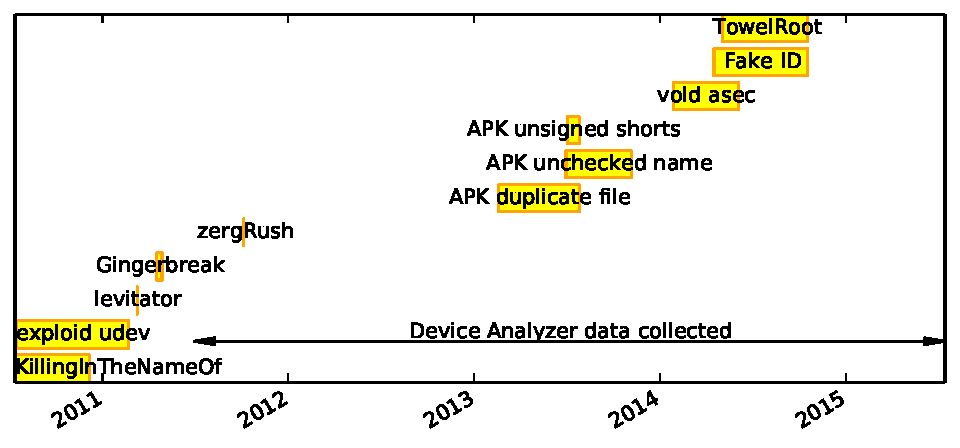
\includegraphics[width=\columnwidth]{figures/vulnerabilities_timeline}
 \caption{Timeline of vulnerabilities. For each vulnerability we show the dates of \textbf{discovery} and, when later, the dates of the first \textbf{fixing release}.}
 \label{fig:vulnerabilities_timeline}
\end{figure}

Figure~\ref{fig:vulnerabilities_timeline} shows the dates of \textbf{discovery} and, when later, the date of the first \textbf{fixing release}.
Some vulnerabilities (\avovuln{levitator}, \avovuln{zergRush}) were fixed in released versions of Android before they were discovered and so are shown as vertical lines, while others were known for months before a version of Android which fixed them was shipped.
During the period in which \da\ data was collected the date when a version of Android with the fix was observed on a \da\ device is taken as the date that version was released.
For vulnerabilities prior to the collection period we estimate the release date using publicly available data.
There is no canonical source of Android release dates, our best guesses and supporting references are available from \avo.

%The discovery dates of our vulnerabilities are not uniform. 
%In particular these data shows a large gap from 2011-10-06 to 2013-02-18 where we do not know of any discoveries of critical vulnerabilities affecting all Android devices.
%The cause of this quiet period is unclear.
%Possible explanations are that: (i) most devices were exposed to known vulnerabilities so there was reason to look for new ones;
%(ii) device manufacturers made it easier to install custom versions of Android, reducing the need for users to root their devices; and
%(iii) device manufacturer specific vulnerabilities (which are not in our analysis here) were easier to find and so attackers looking for vulnerabilities adjusted their focus.


\section{Analysis}
\label{sec:results}
We present the results of our analysis showing that, on average, \daMeanInsecurityPerc\ of Android devices are exposed to critical vulnerabilities and only \daUpdatednessPerc\ run the latest version of Android.
Devices, on average, apply \daUpdatesPerYear\ updates each year, which is less than the rate of critical vulnerability discovery of between \avoVulnsPerYearAllAndroid\ and \avoVulnsPerYear.
\daPercUpdatesDowngrades\ of version changes are downgrades to older versions.
We describe three analyses, examining the vulnerability of Android devices in general (\S\ref{sec:exp:versionsecurity}), explore the upgrade cycle and vulnerability cycle of the ecosystem (\S\ref{sec:exp:android_ecosystem}) and quantify the updates installed on devices (\S\ref{sec:exp:device_updates}).

\subsection{Analysis 1: vulnerability of Android devices}\label{sec:exp:versionsecurity}
\begin{figure}[h]
\centering
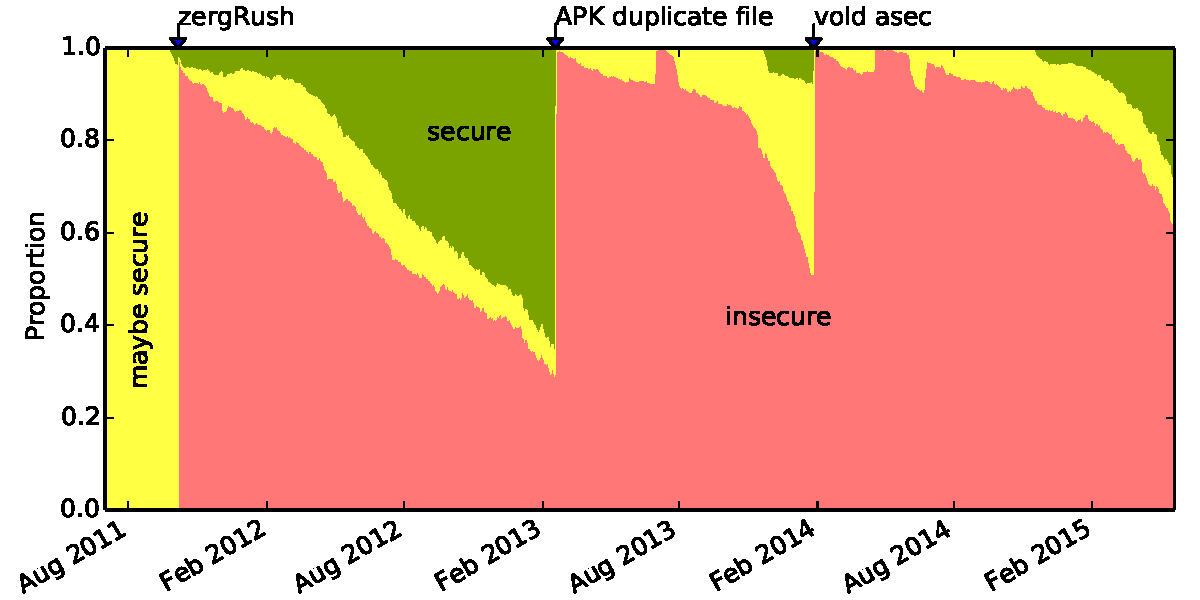
\includegraphics[width=\columnwidth]{figures/proportioninsecure}
\caption{Proportion of devices running insecure, maybe secure and secure versions of Android against time.
The red vertical lines are caused by vulnerabilities being discovered with those which have the biggest impact annotated.
}
\label{fig:proportioninsecure}
\end{figure}
In this analysis we calculate the proportion of Android devices that are exposed to critical vulnerabilities and how that has changed over time.
Figure~\ref{fig:proportioninsecure} describes the proportion of Android devices susceptible to at least one critical vulnerability.

\subsubsection{Method} 
To investigate the vulnerability of Android devices, we used the OS version information from \da\ and the vulnerability data from \avo.
The \avo\ data covers the period from \avoFirstDataDate\ to \avoLastDataDate.
The \da\ data was collected between \daStartDate\ and \daEndDate.
For each device we collected daily version data and any vulnerabilities it was exposed to at that time.
We then normalise these totals for each day by dividing through by the total number of devices with version information on that day.

\subsubsection{Results}

Following time from left to right in Figure~\ref{fig:proportioninsecure} we see all devices are initially \emph{maybe secure} (yellow) since \da\ does not have historical data prior to May 2011. This means we cannot distinguish between devices which are running a version of Android which is known to be vulnerable from one which may have received a backported fix.
This demonstrates the importance of a longitudinal study: this type of analysis requires years of data.
Once \avovuln{zergRush} was discovered in October 2011 then most devices are recorded as \emph{insecure} (red) as they were exposed to that vulnerability.
The remaining devices were already running a version of Android which fixed the \avovuln{zergRush} vulnerability and are therefore marked as \emph{secure} (green).
From October 2011 until the discovery of \avovuln[APK_duplicate_file]{APK duplicate file} in February 2013 the graph shows progressive improvement as devices are upgraded.
This means more and more devices are marked as \emph{secure} because they are now running a secure version of Android, or marked as \emph{maybe secure} because they received an OS update that did not update to a known-good version of Android but which may still have included a backport of a fix, as the update was made available after the vulnerability was disclosed.
From February 2013 onwards regular discovery of critical vulnerabilities ensures that most devices are exposed to known critical vulnerabilities.
This gives us an average exposure to critical vulnerabilities of Android devices of \daMeanInsecurityPerc.

\subsection{Analysis 2: behaviour of the Android ecosystem}\label{sec:exp:android_ecosystem}
In this analysis we examine how the distribution of Android OS versions changes over time and the impact that has on how different vulnerabilities affect the security of Android.
We show that some vulnerabilities continue to have a substantial affect long after they have been fixed and the importance of longitudinal studies for determining whether devices are exposed to a particular vulnerabilities.

\subsubsection{Method} As in Analysis 1, we used the version information for each device to calculate which critical vulnerabilities each device was susceptible to each day.

\subsubsection{Results}
The proportion of devices in the \da\ data running different versions of Android each day is shown in Figure~\ref{fig:norm_os}.\footnote{\label{foot:anomaly}The anomaly beginning in August 2014 is explained in \S\ref{sec:da_changes}.}
It shows how old versions are gradually replaced by new ones, and the long tail of devices which do not see updates to more recent versions.
This gives a mean proportion of devices running the most recent version of Android since 2011 is \daUpdatednessPerc.


\begin{figure}[!h]
 \centering
 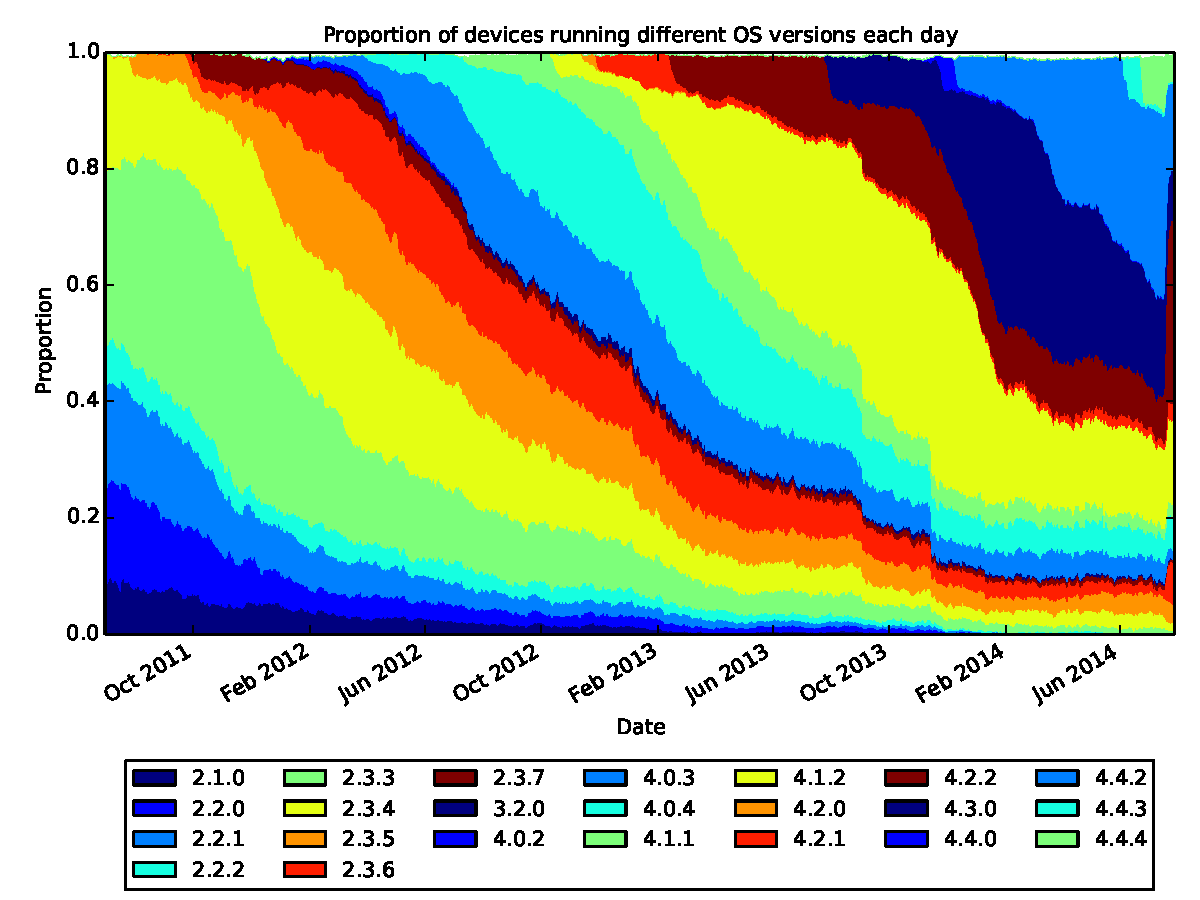
\includegraphics[width=\textwidth]{figures/da_norm_os}
 \caption{Android versions in \da\ data over time.\textsuperscript{\ref{foot:anomaly}}}
 \label{fig:norm_os}
 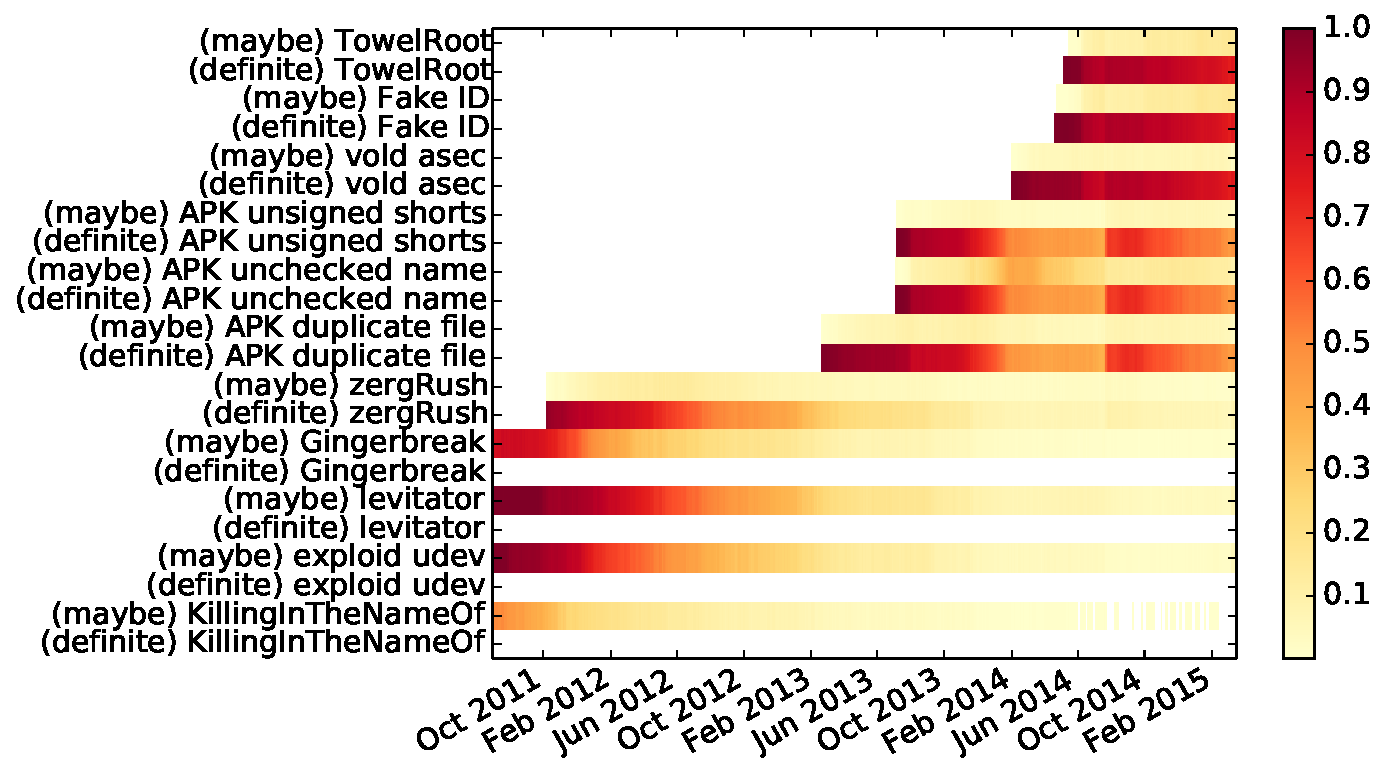
\includegraphics[width=\textwidth]{figures/nvulnerabilities_heat.pdf}
 \caption{Proportion of devices affected by different vulnerabilities. The prefix `(maybe)' indicates `maybe secure' and `(definite)' indicates `definitely insecure'. The first few vulnerabilities are all `maybe secure' as we do not have data from before that vulnerability was discovered while later ones are mostly `definitely insecure' as we know no fixing update reached the devices.
 %The change in behaviour after August 2014 is explained in \S\ref{sec:da_changes}
 \todo{This plot is confusing and perhaps we should quantise the colour map.}
 }
 \label{fig:nvulnerabilities_heat}
\end{figure}

The vulnerabilities devices are exposed to are shown in Figure~\ref{fig:nvulnerabilities_heat}.
For each vulnerability it shows the proportion of devices exposed to that vulnerability and how that changes over time.
The variation of the proportion of devices affected by a vulnerability with time tells us how badly a particular vulnerability affected the Android platform.
In July 2011 the \avovuln[exploid_udev]{exploid} and \avovuln{levitator} vulnerabilities both affect most Android devices, slowly these are fixed as updates roll out and devices are replaced until in January 2013 a much smaller proportion of devices are affected by known vulnerabilities.
However when in February 2013 the first APK signing vulnerability was found which affected all previous versions of Android and even in October 2013 most devices (\daVulnAPKDuplicateFileOctoberPerc) were still vulnerable.
%\begin{figure}%[!b]
%\centering
%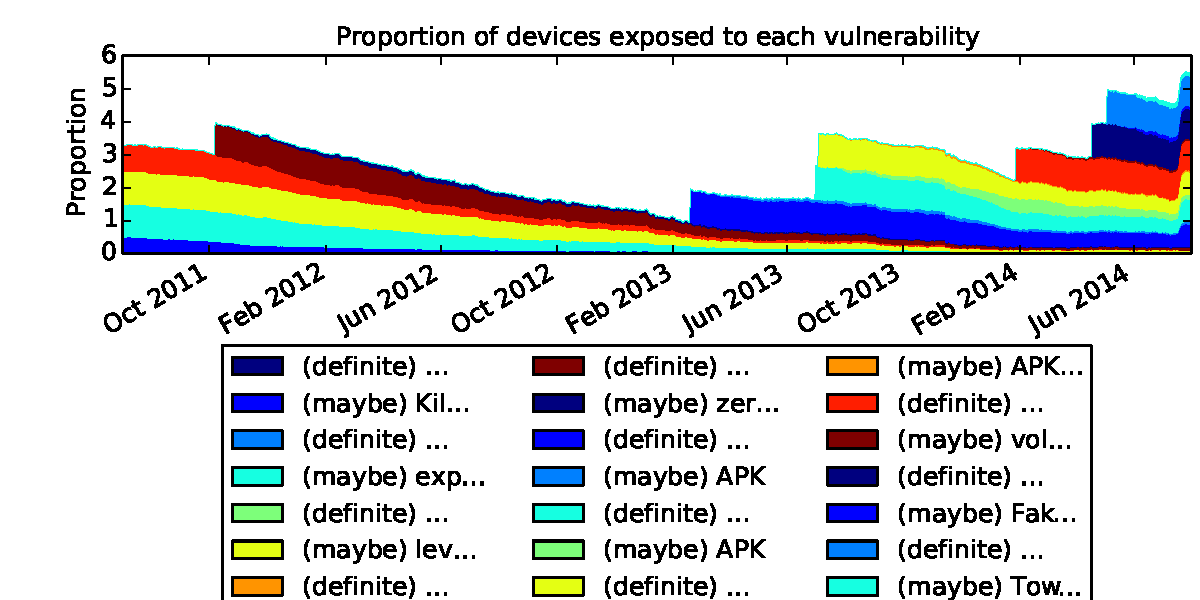
\includegraphics[width=\columnwidth]{figures/vulnerabilities}
%\caption{Proportion of devices exposed to each vulnerability with time (1.0 is 100\%)}
%\label{fig:vulnerabilities}
%\end{figure}

In 2013 three vulnerabilities were found in how Android verified the signatures on APKs.
These are level 2 vulnerabilities in our threat model since they require a new app installation to occur.
Figure~\ref{fig:nvulnerabilities_heat} shows how the the \emph{APK signing vulnerabilities} affected all devices and took months to get fixed for any device.
However what is perhaps more worrying is the long tail on the \avovuln{Gingerbreak}, \avovuln{levitator}, \avovuln[exploid_udev]{exploid} and \avovuln{zergRush} vulnerabilities which are more dangerous level 3 vulnerabilities (since they do not require new app installation) and which affected a significant proportion of devices years later.
%\todo{quantify this long tail and the APK numbers as headline numbers}

\subsection{Analysis 3: Updates to particular devices}\label{sec:exp:device_updates}
Previous graphs summarise data across all the devices, however one of the advantages of the \da\ data is that we can look at what happens to individual devices over time.
This allows us to determine whether newer OS versions are being used because people are buying new phones running newer OS versions or whether existing devices receive updates.

\begin{figure}[!t]
\centering
\begin{subfigure}{\columnwidth}
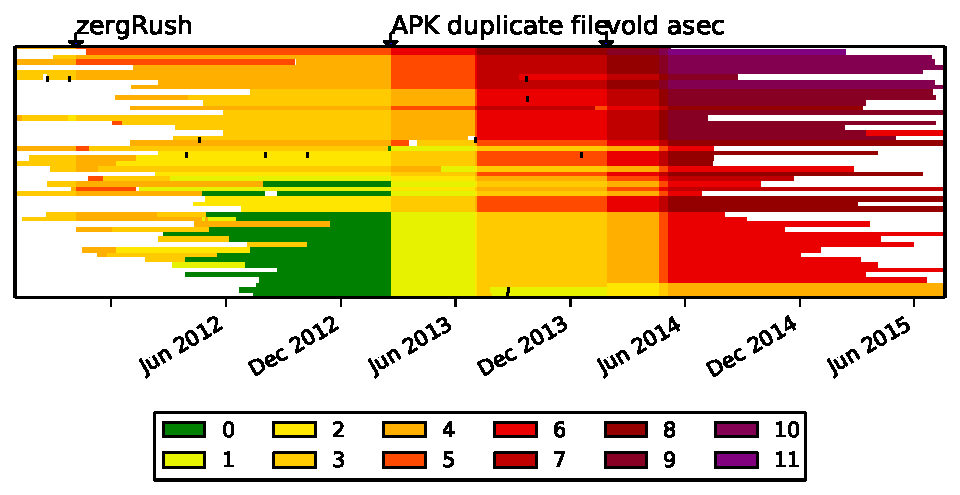
\includegraphics[width=\columnwidth]{figures/device-data-all-security}
\vspace{-1.5em}
\caption{Each strip shows the number of vulnerabilities affecting each device over time.}
\label{fig:device_data_security}
\end{subfigure}
\begin{subfigure}{\columnwidth}
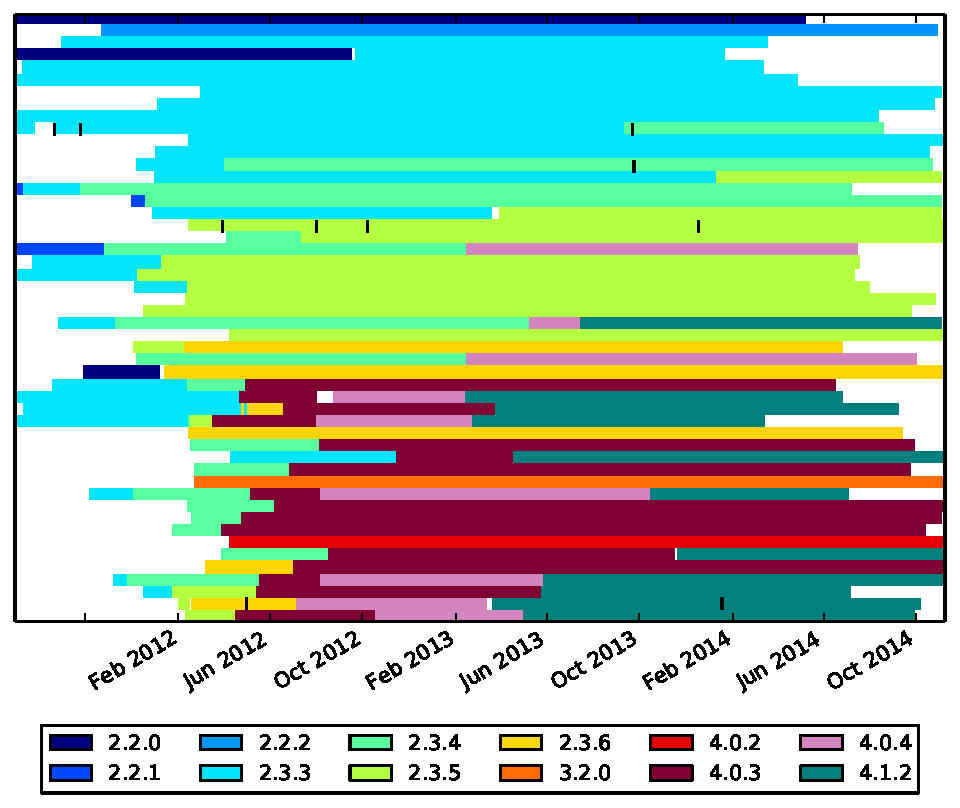
\includegraphics[width=\columnwidth]{figures/device-data-all-os}
\vspace{-1.5em}
\caption{Each strip shows OS versions over time.}
\label{fig:device_data_os}
\end{subfigure}
\caption{The top \daNumDeviceDataDevices\ devices by days of contribution in the \da\ data. One strip per device handset. Black lines show where an update only changed the build number.}
\end{figure}

\subsubsection{Method}
As in Analysis 1, we used the version information for each device to calculate which critical vulnerabilities each device was susceptible to each day.
We also recorded changes in version.
In the \da\ data we have about 1000 devices contributing data in any particular week. \todolater{Use the real average number of devices contributing each week}
However most devices only contribute for a short period of time and so we do not observe updates happening on every device.
Instead we have a hopefully representative sample of updates which happened while \da\ was installed on the devices.
\da\ cannot distinguish between a device being replaced and the \da\ app being removed as while multiple devices can be linked to the same user account, this is a manual process and few users do it.


\subsubsection{Results}
The longitudinal data on the number of vulnerabilities affecting the \daNumDeviceDataDevices\ devices which have contributed the most days of data to \da\ changes over time is shown in Figure~\ref{fig:device_data_security}.
The trend that we saw in Figure~\ref{fig:proportioninsecure} of security improving and then getting worse is also shown here.
It shows how some devices had vulnerabilities, which were fixed, and then further vulnerabilities were discovered, and mostly not fixed.
This implies that these devices had been abandoned by the device manufacturer and were not receiving updates, this is confirmed by Figure~\ref{fig:device_data_os} which shows which OS versions those devices were running.
Some devices start off in 2011 exposed to known security vulnerabilities and are still exposed to those and additional ones in 2014.

We recorded \daNumFullVersionUpdates\ update events and found most are upgrades (\daNumUpdatesUpgrades).
While many upgrades are from one version to the next version there are also a fair number (\daNumUpdatesBigUpgrades, \daPercBigUpgradesNominal) which skip more than \daNumUpdatesSkippedBig\ versions.
Surprisingly there are also a small number of downgrade events (\daNumUpdatesDowngrades, \daPercUpdatesDowngradesNominal) when older versions of Android are installed on to devices.
Possible reasons why users are downgrading are to free up space on their device, to make it easier to root or because a new version introduced bugs.

%The number of devices getting security updates each week, is shown in Figure~\ref{fig:weekly_security_updates}.
%Updates which changed the Android version number so that the number of known vulnerabilities decreased are shown in red.
%Updates which changed the build number but not the version number and so might contain a backported fix for a vulnerability are shown in yellow.
%Updates which did not fix security vulnerabilities (because there were no known security vulnerabilities in the existing version of Android) are shown in green.

By dividing the number of updates observed by the number of device years of data we have collected we compute the number of updates received by a device per year to be \daUpdatesPerYear.
This compares badly with the number of critical vulnerabilities discovered per year of between \avoVulnsPerYearAllAndroid\ (affecting all Android) and \avoVulnsPerYear\ (including the device manufacturer specific ones).

\section{Threats to validity}
\label{sec:validity}
\subsubsection{Comparing \da\ data with the ground truth}
\label{sec:representative}

The data from \da\ we used to investigate the proportion of devices exposed to different vulnerabilities is the OS version.
Unfortunately there is no ground truth of OS version information.
However Google has published API version information almost every month since December 2009 and we have collated this information.\footnote{\url{http://androidvulnerabilities.org/play/historicplaydashboard}}
While API versions are too coarse grained to use for security update detection they are closely related to OS versions and so if the \da\ data on API versions are similar to the Google data on API versions then the \da\ data on OS versions should be representative.
We compared the data from Google and from \da\ and they appear similar, except for the anomaly discussed later.
We analysed the difference between the API version data from \da\ and Google Play, normalising for days since the API version was released.
This shows that the \da\ data systematically overestimates the prevalence of new API versions and underestimates the prevalence of old API versions (except for API version 17 which was particularly popular in a focused study discussed in the next section and so was temporarily overestimated when an old version).
This means that the OS version information from \da\ is likely to be overestimating the prevalence of new OS versions and hence our results are a conservative estimate of the security of Android.
Since most \da\ users are self selecting and install \da\ because they want to find out more about what their phone is doing or to aid research they may be biased and perhaps more likely to install updates.
This allows us to have confidence in the OS version information.
\todolater{we want a statistical metric to claim this strongly with.}


\subsubsection{The effect of focussed studies on \da}
\label{sec:da_changes}
The \da\ data is mostly generated by devices which have the \da\ app installed because their owner happened to come across the app as there has been no advertising and few attempts to increase usage.
However two collaborations with network operators to install \da\ on customer devices resulted in large numbers of new \da\ users coming from particular network operators.
One study was conducted in Norway with 654 installs and one in Bangladesh where 2463 users installed \da.
This latter study is responsible for the sudden change in distribution of OS versions in \da\ beginning in August 2014 in Figures \ref{fig:proportioninsecure}, \ref{fig:norm_os} and \ref{fig:nvulnerabilities_heat} as for that period Bangladeshi users contributed over half of the \da\ data.
%We could normalise out the influence of the Bangladeshi users, however they are Android users too and they also need security updates.
To investigate the sensitivity of our results to the Bangladesh study we truncated our data before this study started and found the percentage of vulnerable devices to be 85.6\% rather than \daMeanInsecurityPercNominal, the percentage of devices running the latest version to be 5.71\% rather than \daUpdatednessPercNominal\ and the number of updates per year to be 1.48 rather than \daUpdatesPerYearNominal.
Hence removing this anomaly would have no effect on our main conclusions.

\subsubsection{The selection of vulnerabilities in \avo}
We have not included all the vulnerabilities from \avo. 
In particular, we have not included any device manufacturer specific vulnerabilities, even when these are widespread (such as vulnerabilities in Qualcomm\footnote{Qualcomm is particularly good at publicly disclosing vulnerabilities and the patches which fix them. \url{https://www.codeaurora.org/projects/security-advisories/}} chipsets) because it is difficult to work out which devices are affected.
There also tends to be less public information available about manufacturer-specific vulnerabilities which makes them harder to tie down.

For some other vulnerabilities which might affect all Android devices it is hard to work out which devices are affected.
For example, \avovuln[pty_race]{pty race} is a Linux kernel vulnerability. We found 48 commits which fixed this vulnerability on different branches. On some branches it was also accidentally fixed, and later reintroduced, before finally being fixed properly, and therefore determining which devices were vulnerable relies on knowing where, and on which branch, the kernel code for a specific release was taken from.

For some vulnerabilities the required patch is not in AOSP.
This is despite the fact that some device manufacturers have shipped builds containing the fix.
This makes it difficult to determine whether a specific device is vulnerable.
For \avovuln[RageAgainstTheCage_adb]{RageAgainstTheCage adb} and \avovuln[keystore_buffer]{keystore buffer} vulnerabilities we do not have sufficient data to determine whether they fit one of our attack vectors as the former may require physical ADB access and the latter may be thwarted by the sandbox.
However a sensitivity analysis showed that those two vulnerabilities make little difference to our results.

\subsubsection{Limitations}
We still do not know where new versions of Android come from.
Over time newer versions of Android come to dominate, but the proportion due to new phone purchases verses the proportion due to updates of existing devices is unknown.
Device Analyzer is the only available large data set we know of with longitudinal traces of Android OS version strings.
Unfortunately this data set only records \daNumUpdatesUpgrades\ upgrades which, broken down over \daOSMonthsOfData\ months and \daNumSigOSVersions\ OS versions is only \daUpdatesPerMonthPerVersion\ updates per version per month. This is not enough to build a statistically significant prediction of the expected transition between versions of Android.
If manufacturers shipped security updates without changing the build number then we would not be able to detect this, but that would indicate a level of incompetence likely to damage security.

 
\section{Related work}
\label{sec:related}
Using the methods and data described in this paper we have determined that, on average, \daMeanInsecurityPerc\ of devices were exposed to known critical vulnerabilities between 2011 and 2015.
Felt et al.\ studied 6 Android handsets in 2011 and found they were exposed to root vulnerabilities at least 74\% of the time~\cite{Felt2011}.
Our approach differs from their study because they used data from 6 handsets and assumed the best possible update distribution, while our work is based on a large sample of devices tracking the actual update distribution.
Nevertheless, our own analysis as well as comparison with their work suggests protection against critical vulnerabilities has not improved significantly over the last 4 years. 
Felt et al.\ also found that 4 of the 46 malware samples (8\%) they analysed contained root exploits, much lower than rates found in later (larger) studies which found rates of 36.7\%~\cite{Zhou2012b} and 40\%~\cite{Zhou2012a} in 2012.

Currently, finding and exploiting vulnerabilities is typically a time-consuming manual process.
Therefore an attacker has to invest significant human resource to first find a bug and then write code to exploit the vulnerability.
To reduce the effort involved in finding a bug, attackers can look at security-related commits made to open source repositories.
Attackers have taken this approach for the Firefox web browser~\cite{Barth2011}.
Google does not release updates to the Android source code until after the release of the relevant update~\cite{AndroidSecurity2014}.
This reduces the time available for an attacker to exploit a vulnerability by looking at security updates disclosed in the source code repository.
Reducing it from, the interval between the commit of the first fix and the fix being deployed to most devices, to the interval between the first fixing release and the fix being deployed to most devices; unfortunately this can still take months or years.
For example, the zergRush vulnerability was fixed in a release before it was publicly discovered but it still took 27 months for 90\% of the devices in our study to be definitely fixed\footnote{Definitely fixed is 1 $-$ (definitely insecure + maybe secure), maybe fixed is 1 $-$ definitely insecure} (25 months for 90\% of devices to be maybe fixed).

Brumley et.\ al. has shown it is possible to automatically generate exploits from binary fixes, for example by using security updates issued by manufacturers~\cite{Brumley2008}. 
Similarly, the Woodpecker tool automatically finds permission leaks in stock Android phone images~\cite{Grace2012}.
Once such automated techniques mature, it will become even more important to provide security updates promptly to every Android device in the ecosystem because an attacker can turn the contents of a released fix into an exploit in a matter of minutes or hours.

Security in depth is also a useful strategy.
In this regard, iOS provides additional safeguards beyond those used in Android, including a pre-distribution review, mandatory code-signing by the manufacturer, and (with the important exception of ROP-based attacks~\cite{Wang2013a}) the technical prohibition of dynamic code loading by an app.
These features, as well as Address Space Layout Randomisation (ASLR) and mandatory access controls, has resulted in a lower level of malware affecting iOS when compared to Android~\cite{Felt2011}.

There are continuing efforts to reduce the impact of critical vulnerabilities, both in Android and elsewhere.
SEAndroid~\cite{Smalley2013} which is included in Android from version 4.1~\cite{jelly-bean-release} and fully enforcing from version 5.0~\cite{AndroidSecurity2014} claimed to prevent some root vulnerabilities and to reduce the impact of others.
Capability based enforcement systems such as Capsicum~\cite{Watson2010} substantially reduce the capabilities that an exploit has to try and gain increased privilege with and could be included in Linux\footnote{\url{https://github.com/google/capsicum-linux}} and hence Android.

Rather than fixing critical vulnerabilities, security can be obtained by detecting malicious apps and preventing their installation or execution.
Detection strategies include RiskRanker, which classified 3\,281 out of 118\,318 apps (2.8\%) as risky of which 718 (22\%) were malware and 322 (10\%) were previously unknown malware, an infection rate of 0.6\% across multiple markets~\cite{Grace2012a}.
DroidRanger also analysed apps finding 148 out of 182\,823 apps (0.08\%) to be malicious across multiple markets of which 29 were previously unknown~\cite{Zhou2012a}.
%DroidRanger: It used permission-based behavioural fingerprinting which looked at the permissions of known malware and heuristic-based filtering -- dynamic loading of both Dalvik and native code.
A common technique used by attackers is to include malicious code in repackaged popular apps. 
AnDarwin uses this insight to detect similar apps, and found 169 out of 265\,359 of all apps studied (0.06\%) were malicious clones~\cite{Crussell2013}.
%AnDarwin: It used clustering based on semantic vectors derived from the program dependence graphs to detect similar apps.

Unfortunately, whilst these tools were successful in finding malware, such techniques are not perfect.
The Malware Genome project collected 1\,260 malware samples from 2010--2011~\cite{Zhou2012b} and found a best case anti-malware detection rate of 79.6\%.
Similarly, DroidChameleon found that anti-virus products could not detect malware if the binary was automatically permuted~\cite{Rastogi2013}.
Therefore detecting risky apps which might contain critical vulnerabilities is a useful tool, but it does not replace the need to provide security updates.

%All these app analysis projects have been hampered by the difficulty of obtaining full datasets of Android apps as Google does not make these available (and researchers who automatically download them violate Google's Terms of Service).
%PlayDrone was a particularly effective project which circumvented Google's protective measures and downloaded over 1\,100\,000 apps from Google Play, allowing an in depth analysis~\cite{Viennot2014}.


The percentage of Android devices running the most recent version (\daUpdatednessPerc) compares unfavourably with the rate ($>90$\%) for Windows XP SP2 computers contacting the Microsoft update servers~\cite{Gkantsidis2006}.
A simple numerical comparison is unfair because only one major OS version was considered in the Microsoft analysis, and data was only collected from computers which contacted the update server, although this was the default.
More recent data demonstrates the difficulty of upgrading computers between major OS versions, with 27\% of Windows computers running Windows XP in July 2014,\footnote{\url{https://archive.today/PLGxn}} four months after Windows XP stopped receiving security updates.



\section{Conclusion}
\label{sec:conclusion}
We have described the three levels of defence provided to Android users today and determined that the app sandbox is the best place to prevent malware from gaining root.
However the latency in the security update process means that on average \daMeanInsecurityPercNominal\ of Android devices are exposed to known critical vulnerabilities which break out of the sandbox and only \daUpdatednessPercNominal\ of devices run the latest version of Android.
Devices apply \daUpdatesPerYearNominal\ updates each year less than the rate of critical vulnerability discovery of between \avoVulnsPerYearAllAndroidNominal\ and \avoVulnsPerYearNominal.

Installing regular updates is the best defence against malware, however, as we have shown, these updates are rarely forthcoming. 
Therefore Android users need to take additional steps to protect themselves. 
Firstly, users should only install apps from Google Play, which has been shown to have a lower level of malware than third-party markets and is known to contain static and dynamic analysis of available apps.
Secondly, users should enable the Google Verify Apps feature if available or use an anti-malware app. 
Thirdly, users should avoid using untrusted WiFi networks or use them in conjunction with a VPN tunnel to a trusted network. 
Finally, if the user is running a device with API level 17 or above and is able to determine the target API version of their apps, they should consider uninstalling all apps with a target API of less than 17.

In the long term, there needs to be greater emphasis on providing timely updates.
This could be fixed through a variety of mechanisms.
Increased regulation is one potential solution.
Currently manufacturers do not even provide updates for the length of the contracts under which the users originally bought the phone, despite efforts by the ACLU to persuade the FTC to force them to do so~\cite{Soghoian2013}, and despite the FTC forcing HTC to do so~\cite{FTCHTC2013}.

Alternatively, decentralised management might work.
The claim of the open source software `bazaar' is that it is more secure because anyone can review the source code and provide fixes~\cite{Raymond1999}.
On the surface, Android is an open source project, and therefore others should be able to step in when the manufacturer fails to provide timely updates.
Unfortunately only manufacturers can provide updates today because the complete source code for the (often modified) operating system, as well as the drivers and the build environment, are not available for many devices.
This is unlikely to change since there are economic disincentives from the manufacturers' perspective, and in any case there is a trust issue which needs to be solved: how does the user determine whether a binary from an alternative supplier is more secure than the one they already have installed?

The fundamental problem is really one of a misalignment of incentives in the current Android ecosystem: there are too few reasons why manufacturers should provide timely security updates.
A more rigid vertically integrated marked would likely improve the security of Android at the cost of some of the freedom it current affords manufacturers and users.

\identifying{
\section*{Acknowledgements}
Thanks to: Richard Clayton, the mobile security reading group and Anil Madhavapeddy for reading drafts;
David Robertson for statistical advice;
and Laurent Simon, Thomas Coudray, Adrian Taylor, Justin Case, Giant Pune and Khilan Gudka for reporting vulnerabilities.
We were funded by the EPSRC and Google but the the work presented here does not necessarily reflect their views.
}

\printbibliography



\end{document}
